%%% PLOT FILE - Choice of a robotic partner
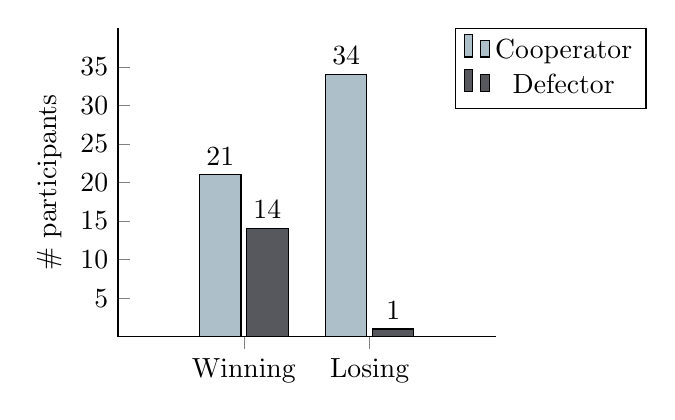
\begin{tikzpicture}%
\begin{axis}[%
    ybar,
    %title=Test,%
    axis y line*=left, axis x line*=bottom,%
    ymin=0,
    ymax=40,
    ytick={5,10,...,35},
    legend style={at={(1.4,1)}},
    %x tick label style={rotate=45,anchor=east},%
    symbolic x coords={Winning, Losing},%
    xtick=data,
    enlarge x limits=1,
    height=5.5cm,
    bar width=15pt,
    ylabel=\# participants,%
    nodes near coords,
        ]%
\addplot+[
    color=black, %
    fill={rgb,255:red,173; green,192; blue,202},%
    %postaction={pattern=crosshatch dots},
    %error bars,
    y dir=normal,
    %y explicit
    ]
				coordinates {
            (Winning,21.0)
            (Losing,34.0)
				};
\addplot+[%
    color=black, %
    fill={rgb,255:red,87; green,87; blue,94},%
    %error bars/.cd,%
    y dir=normal,%
    %y explicit,%
        ]%
coordinates {
            (Winning,14.0)
            (Losing,1.0)
        };%
\legend{Cooperator,Defector}
\end{axis}%
\end{tikzpicture}%